\section{Situaciones de la vida real que pueden ser modeladas con el problema del Camino acotado de costo minimo}
\subsection{Viaje en ruta: Minimizar la distancia de viaje dada una cantidad fija de dinero}
Sea G = (V, E) un grafo simple, se quiere modelar un mapa de ciudades y rutas entre ellas, para ello vamos a definir V el conjunto de nodos donde cada nodo representa una ciudad en el mapa. Asimismo, E ser\'a el conjunto de aristas en donde, sean $v_1,v_2 \in V $ entonces $\exists $ $(v_1,v_2) \in E \Leftrightarrow$ existe una ruta entre las ciudades $v_1$ y $v_2$. Definiremos a continuaci\'on dos funciones sobre el conjunto E de aristas tales que:
\begin{itemize}
	\item $f:E \rightarrow \mathbb{R}_+$: funcion asociada a la distancia entre $v_1$ y $v_2$.
	\item $g:E \rightarrow \mathbb{R}_+$: funcion asociada al costo de viajar entre $v_1$ y $v_2$.
\end{itemize}
Sea ademas $k \in \mathbb{R}_+$ el dinero del que se dispone para realizar el viaje, el objetivo de esta situacion es, dados $v_1, v_2 \in V$ se quiere llegar de la ciudad $v_1$ a la ciudad $v_2$ minimizando la distancia del viaje, pero se debe poder cubrir el costo total del viaje con la cantidad $k$ de dinero disponible.\\
El la siguiente figura se ve un ejemplo de como podria ser un grafo de estas caracteristicas, ade\'as se ve que el camino mas corto en respecto de la funcion distancia $f$, no necesariamente
cumple el requisito de estar dentro de la cota respecto a la funcion de costo $g$ y el dinero disponible $k$. Los pares ordenados en las aristas indican (f: distancia, g: costo).\\

\begin{figure}[H]
	\centering
	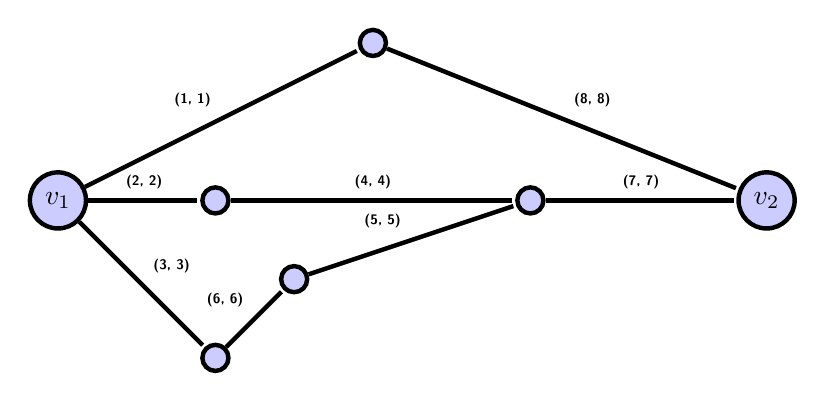
\begin{tikzpicture}[shorten >=1pt, auto, node distance=3cm, ultra thick,
   edge_style/.style={draw=black, ultra thick,font=\sffamily\tiny\bfseries}]
	  \node [circle,draw=black,fill=blue!20] (n1) at (1,2) {$v_1$};
	  \node [circle,draw=black,fill=blue!20] (n2) at (5,4)  {};
	  \node [circle,draw=black,fill=blue!20] (n3) at (3,2)  {};
	  \node [circle,draw=black,fill=blue!20] (n4) at (3,0)  {};
	  \node [circle,draw=black,fill=blue!20] (n5) at (4,1)  {};
	  \node [circle,draw=black,fill=blue!20] (n6) at (7,2)  {};
	  \node [circle,draw=black,fill=blue!20] (n7) at (10,2) {$v_2$};

	  \foreach \from/\to/\distance/\cost in {n1/n2/1/1, n1/n3/2/2, n1/n4/3/3, n3/n6/4/4, n5/n6/5/5, n4/n5/6/6, n6/n7/7/7, n2/n7/8/8}
	    %\draw (\from) -- (\to);	    
	    \draw [edge_style] (\from) edge node{(\distance, \cost)} (\to);

	\end{tikzpicture}
	\caption{Ejemplo de conexion entre ciudades.} \label{fig:vida_real_1}
\end{figure}

El camino mas corto seria ... pero vemos que con esos pesos se pasa de K ... entonces el mejor camino acotando el costo por K es ...

\subsection{Camino mas conveniente segun relieve: Expedicion en la colina}
Otra posible aplicacion para este problema es la siguiente situacion. Se quiere ir de un punto A a otro B donde existe una zona con un relieve complicado, una colina, en el medio de estos 2 puntos, hay varios caminos que pueden tomarse, cada uno de ellos tiene un costo asociado a la cantidad en litros de nafta requerida para atravesar ciertos sectores de la zona dado su relieve y tambien tiene otro valor asociado, que es el tiempo que toma llegar de A hasta B. El objetivo es llegar de A hasta B en el menor tiempo posible, teniendo en cuenta una cota de K litros en la nafta de la que se dispone. Sea G = (V, E) un grafo simple, el conjunto V de nodos denota por cada nodo un sector de la zona a atravesar y el conjunto de aristas E establece la siguiente relacion: Sean $v_1,v_2 \in V $ entonces $\exists $ $(v_1,v_2) \in E$ de peso $ (t, l) \in \mathbb{R_+}^2 \Leftrightarrow$ existe un sendero entre los sectores $v_1$ y $v_2$ con costo de l litros de nafta que toma t minutos en ser recorrido.